% Created 2016-02-12 Fri 13:24
\documentclass{scrartcl}
\usepackage[utf8]{inputenc}
\usepackage[T1]{fontenc}
\usepackage{fixltx2e}
\usepackage{graphicx}
\usepackage{longtable}
\usepackage{float}
\usepackage{wrapfig}
\usepackage{soul}
\usepackage{textcomp}
\usepackage{marvosym}
\usepackage{wasysym}
\usepackage{latexsym}
\usepackage{amssymb}
\usepackage{hyperref}
\tolerance=1000
\usepackage{khpreamble}
\providecommand{\alert}[1]{\textbf{#1}}

\title{Computerized control - Partial exam 1 (20\%)}
\author{Kjartan Halvorsen}
\date{2016-02-10}
\hypersetup{
  pdfkeywords={},
  pdfsubject={},
  pdfcreator={Emacs Org-mode version 7.9.3f}}

\begin{document}

\maketitle



\section*{Instructions}
\label{sec-1}


Write your answers clearly and motivate well! You can write by hand or on a computer. If you write by hand, you may scan your pages using, for instance, the app CamScanner that can produce pdf-documents. \textbf{Answers should be handed in on Blackboard (assignment ``Partial exam 1'') no later than midnight 2016-02-11.}
\section*{The plant}
\label{sec-2}

The dynamic model of a particular industrial induction motor\footnote{Jung, Seul, and Richard C. Dorf. ``Analytic PIDA controller design technique for a third order system.'' Decision and Control, 1996., Proceedings of the 35th IEEE Conference on. Vol. 3. IEEE, 1996.
 } can be written
\begin{equation}
G(s) = \frac{168}{s(s^2 + 25.9s + 168)}
\label{eq:plantmodel}
\end{equation}
\section*{Problem 1 (10p)}
\label{sec-3}

  Determine the poles of the continuous-time model and plot these in the imaginary plane.
\section*{Problem 2 (50p)}
\label{sec-4}

  Obtain a sampled model of the plant in \eqref{eq:plantmodel} using zero-order-hold sampling for arbitrary $h$ (sample the model symbolically). You may express the pulse-transfer function as a sum of rational functions in $z$ (you do not have to write it on a common fraction line). 
  
\section*{Problem 3 (10p)}
\label{sec-5}

  Choose a reasonable value for the sampling period $h$, considering the poles of the plant $G(s)$, and using the rule-of-thumb in Åström \& Wittenmark section 2.9.
\section*{Problem 4 (20p)}
\label{sec-6}

  Determine the poles of the discrete-time system using the sampling period you decided in Problem 3. Plot the poles in the imaginary plane. For each pole, indicate which continuous-time pole it corresponds to.
\section*{Problem 5 (10p)}
\label{sec-7}

  The unit delay in discrete-time has pulse-transfer function \[H(z) =\frac{1}{z}\] with a single pole in the origin. Where is the pole of the corresponding continuous-time system? 
\section*{Solutions}
\label{sec-8}
\subsection*{Problem 1}
\label{sec-8-1}

   The continuous-time poles are
   \begin{center}
   %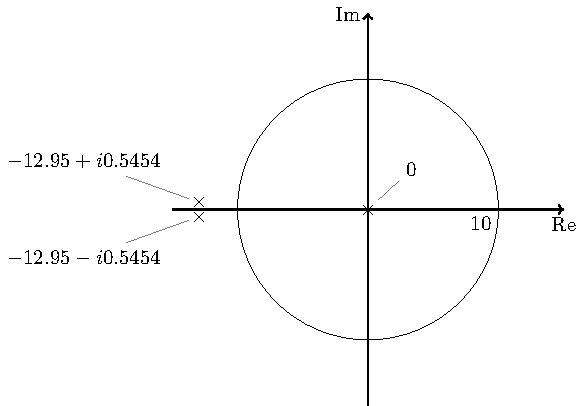
\includegraphics[width=0.5\linewidth]{ct-poles}
   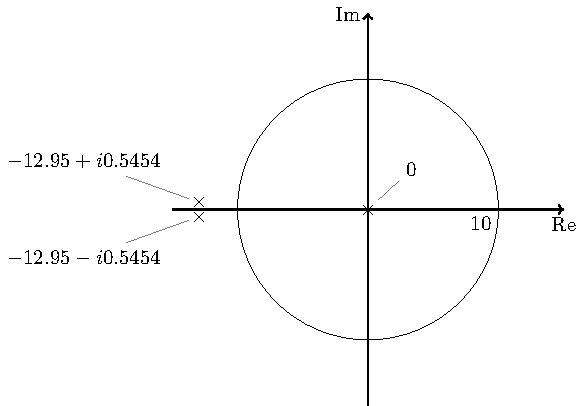
\includegraphics[]{ct-poles}
   \end{center}
   
\subsection*{Problem 2 - Sampled model}
\label{sec-8-2}
\subsubsection*{1}
\label{sec-8-2-1}

  Find the step-response in the Laplace-domain by partial fraction decomposition. This gives (with the help of a symbolic math tool)
       \begin{equation*}
        \begin{split}
         Y(s) &= \frac{G(s)}{s} = \frac{168}{s^2(s^2 + 25.9s + 168)}\\
              &= \frac{1}{s^2} - \frac{0.15417}{s} + \frac{0.15417s + 2.993}{s^2 + 25.9s + 168}.
        \end{split}
       \end{equation*}
      The last term can be written on the form 
      \[ \frac{0.15417s + 2.993}{s^2 + 25.9s + 168} = b_1\frac{s+a}{(s+a)^2 + \omega^2} + b_2\frac{\omega}{(s+a)^2 + \omega^2}, \] 
      with
      \[ a = 12.95, \quad \omega=0.5454. \]
      \[ b_1 = 0.15417, \quad b_2 = 1.8269\]
      We can then use the formulas for the laplace-transform of exponentially decaying sine- and cosines
      \[ \mexp{-at}\cos(\omega t) \quad \underset{\longleftrightarrow}{\mathcal{L}} \quad \frac{s+a}{(s+a)^2 + \omega^2} \]
      \[ \mexp{-at}\sin(\omega t) \quad \underset{\longleftrightarrow}{\mathcal{L}} \quad \frac{\omega}{(s+a)^2 + \omega^2} \]
\subsubsection*{2.}
\label{sec-8-2-2}

    Apply the inverse laplace transform on each of the terms to get $y(t)$:
       \begin{equation*}
        \begin{split}
         y(t) &= \laplaceinv{Y(s)} = \laplaceinv{\frac{1}{s^2}} - \laplaceinv{\frac{0.15417}{s}} \\
              & \quad + \laplaceinv{0.15417\frac{s+12.95}{(s+12.95)^2 + 0.5454^2}}\\
              & \quad + \laplaceinv{1.8269\frac{0.5454}{(s+12.95)^2 + 0.5454^2}}\\
              &= tu(t) - 0.15417u(t) + 0.15417\mexp{-12.95t}\cos(0.5454t) + 1.8269\mexp{-12.95t}\sin(0.5454t).
     \end{split}
    \end{equation*}
\subsubsection*{3.}
\label{sec-8-2-3}

    Sample and apply z-transform
   The sampled step-response becomes (note that $u(kh) = u(k)$)
    \begin{equation*}
     \begin{split}
      y(kh) &= hku(k) - 0.15417u(k) + 0.15417\left(\mexp{-12.95h}\right)^k\cos(0.5454hk) + 1.8269\left(\mexp{-12.95h}\right)^k\sin(0.5454hk).
     \end{split}
    \end{equation*}
   From the table of z-transforms we get
    \begin{equation*}
     \begin{split}
      Y(z) &= \frac{hz}{(z-1)^2} - \frac{0.15417z}{z-1} \\
           &\; + 0.15417 \frac{z(z-\mexp{-12.95h}\cos(0.5454h))}{z^2 - 2\mexp{-12.95h}\cos(0.5454h)z + \mexp{-2\cdot{}12.95h}}\\
           & \quad + 1.8269 \frac{z\mexp{-12.95h}\sin(\0.5454h)}{z^2 - 2\mexp{-12.95h}\cos(0.5454h)z + \mexp{-2\cdot{}12.95h}}.
     \end{split}
    \end{equation*}
\subsubsection*{4}
\label{sec-8-2-4}

    Divide by $U(z) = \frac{z}{z-1}$
       \begin{equation*}
        \begin{split}
         H(z) &= \frac{Y(z)}{U(z)} = \frac{h}{z-1} - 0.15417\\
              &\; + 0.15417 \frac{(z-1)(z-\mexp{-12.95h}\cos(0.5454h))}{z^2 - 2\mexp{-12.95h}\cos(0.5454h)z + \mexp{-2\cdot{}12.95h}}\\
              &\quad + 1.8269 \frac{(z-1)\mexp{-12.95h}\sin(\0.5454h)}{z^2 - 2\mexp{-12.95h}\cos(0.5454h)z + \mexp{-2\cdot{}12.95h}}\\
      &= \frac{h-0.15417z + 0.15417}{z-1}\\ &\; + \frac{(z-1)\big(0.15417(z-\mexp{-12.95h}\cos(0.5454h)) + 1.8296\mexp{-12.95h}\sin(\0.5454h)\big)}{(z-\mexp{-12.95h}\cos(0.5454h))^2 + \mexp{-12.95h}\sin^2(0.5454h)}.
        \end{split}
       \end{equation*}
\subsection*{Problem 3 - choose sampling period}
\label{sec-8-3}

   The dynamics of the system is governed by the two complex-conjugated poles. These are almost completely damped, with 
   \[ \zeta = \frac{12.95}{\sqrt{12.95^2 + 0.5454^2}} \approx 0.999. \]
   and
   \[ \phi = \cos^{-1}(\zeta) = 0.042. \] 
   This gives for the epxression for rise time of a second order system (Å\&W 2.9)
   \[ T_r \approx \omega_0^{-1}\mexp{\phi/\tan(\phi)} = \omega_0^{-1}2.72. \]
   It is suitable with 4-10 sampling periods per rise time. This gives
   \[ (4-10)h \approx \omega_0^{-1}2.72 \]
   or
   \[ h \approx \omega_0^{-1} (0.272 - 0.68) \]
   with 
   \[ \omega_0 = \sqrt{0.5454^2 + 12.95^2} = 12.96 \]
   \[ h \approx 0.021 - 0.052. \]
\subsection*{Problem 4 - plot the discrete-time poles}
\label{sec-8-4}

   With \(h=0.025\) the poles are 
   \begin{align*}
   z_1 &= \mexp{-12.95h}\cos(0.5454h) + i\mexp{-12.95h}\sin(0.5454h) \approx = 0.723 + i0.010\\
   z_2 &= \mexp{-12.95h}\cos(0.5454h) - i\mexp{-12.95h}\sin(0.5454h) \approx = 0.723 - i0.010\\
   z_3 &= 1
   \end{align*}
   and  plotted below
   \begin{center}
   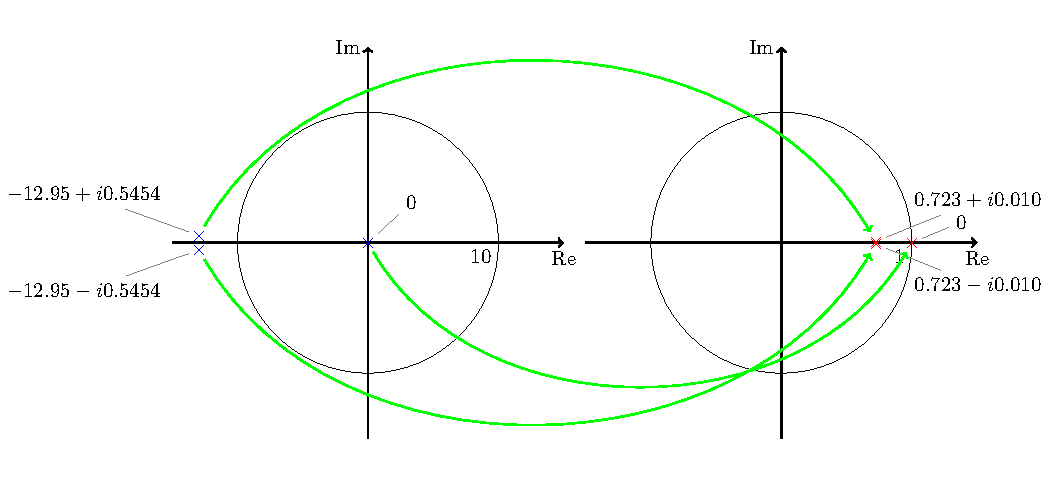
\includegraphics[width=0.8\linewidth]{dt-poles}
   \end{center}
\subsection*{Problem 5 - pole of the continuous-time delay}
\label{sec-8-5}

   The pole of a transfer function $G(s)$ is a value of $s$ for which the value of the transfer function goes to infinity. The continuous-time transfer function corresponding to a unit delay in discrete time (delay of $h$) is 
   \[ G(s) = \mexp{-sh}. \]
   The value of the transfer function goes to infinity as \( s \to -\infty\). Hence the pole is at minus infinity.

   Or, in other words a pole at minus infinity is mapped to zero through the mapping 
   \[ z = \mexp{sh} \]
   that relates continuous- and discrete-time poles.

\end{document}
